% -*-LaTeX-*-

\section{Personal Clouds}
\label{sec:model}

\subsection {Existing Models}

As we are writing, new services are being introduced to the
market : they are distributed storage systems, with support for
disconnected operations. A local copy of the files is kept on every
device participating in the system. These products results in a user
experience close to what we are aiming at with pFS. Nevertheless, these
systems rely on the existence of a central server, always available,
where conflicts are detected. Figure \ref{OthModel} shows a diagram of
such existing solutions.

\begin{figure}[ht]
\begin{center}
  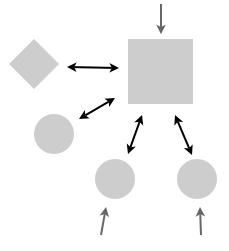
\includegraphics [scale=0.4] {img/other_model}
  \caption{\label{OthModel}
    {\small Existing models : cloud infrastructure with local
      caches. The circles represent high capacity devices, the diamond
      represents a mobile devices as smartphones or digital players,
      and the square represents the cloud infrastructure always
      available, in charge of resolving conflicting updates. Black
      arrows represent the connection and update propagation patterns
      while the grey arrows represent updates made to the user data.}}
\end{center}
\end{figure}

Unfortunately, we believe that the need for a central server has a few
drawbacks. The end-user has to trust the company providing the cloud
infrastructure for storing \emph{all} his data. Such models might
result into closed infratstructes tighted to the storage cloud
they rely on, where compatibility or migration between different
service providers might become difficult.

\subsection {pFS Personnal Cloud Model}

It appears that mobile devices (PDAs, smartphones, digital audio
players) with connectivity (Wifi, BlueTooth, Wire) carried by users
wherever they go, can be used as a substitute to an always available
central infrastructure for update propagation. The connection patterns
between users devices and their mobile devices appear to be as
frequent and efficient as the ones offered by a central
infrastructure.

Based on this observation, our main contribution, is the design of a
flexible versioning system that does not rely on the existence of a
central server, where conflicts are resolved on every devices
participating in the system. Such versioning allows update propagation
between any couple of devices participating in the system. In such
framework, users' mobile devices, even if considered as any other
devices by the system, become a very frequent update relay between the
users' other devices. Figure \ref{PfsModel} shows a diagram of pFS model.

\begin{figure}[ht]
\begin{center}
  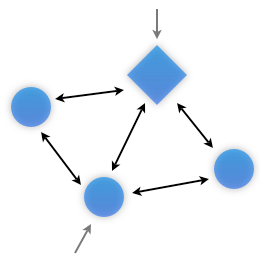
\includegraphics [scale=0.4] {img/pfs_model}
  \caption{\label{PfsModel} {\small pFS model : personnal
      cloud. Updates are propagated between any couple of
      devices. The mobile devices appear as efficient relays 
      for updates.}}
\end{center}
\end{figure}


Our intend with pFS is to provide a distributed storage system where
data is cached locally on every devices and updates seamlessly
propagated asynchronously. Such ``personnal cloud'' can provide the
location independent layer needed to overcome the management hassle
incurred by the growing number of devices a user has to deal with on a
daily basis.

We think that such personnal clouds should complement the use of
remote computing and storage clouds. The principles we expose are
compatible with the use of remote servers as nodes in one's personnal
cloud for providing services that are not available on conventional
devices, such as online (Web-based) access and modification of data.

Our model of ``personnal cloud'' can also be used to spawn devices
owned by multiple users to ease the collaboration process on files that
otherwise need to be sent back and forth between the participants.

pFS also provides a solution to back-up since chances are low
for someone to loose all of its devices at the same time. Even if the
mobile device is used as a way to propagate updates, their loss does not
jeopardize the system since all the data is present on the last device
that connected with it. 

Finally, the goal of pFS is to provide a distributed storage system
where the user data is available on all his devices, and the updates
he makes follow him on the mobile devices he always carry with him. It
provides access to up-to-date versions of any ressource without
relying exclusively on a centralized, potentially untrusted (doubtly
free) infrastructure. 


\subsection {Mobile Devices}

In the following sections, we assume mobile devices as smartphones and
digital player have enough storage capacity for holding all of a
user's data. This might become true in a near future but is certainly
not today. We acknowledge this fact and leave as future work the
design of a caching policy for the mobile devices. Please refer to
section \ref{sec:futwk} for a more extensive discussion of this issue.


% Local Variables:
% tex-main-file: "main.ltx"
% tex-command: "make;:"
% tex-dvi-view-command: "make preview;:"
% End:
